\documentclass{article}
\usepackage[utf8]{inputenc}
\usepackage[spanish]{babel}
\usepackage{listings}
\usepackage{graphicx}
\graphicspath{ {images/} }
\usepackage{cite}

\begin{document}

\begin{titlepage}
    \begin{center}
        \vspace*{1cm}
            
        \Huge
        \textbf{Parcial 1}
        
        \textbf{Informe de desarrollo}
            
        \vspace{0.5cm}
        \LARGE
        Informática II
            
        \vspace{1.5cm}
            
        \textbf{Reinaldo Marín Nieto}


        \textbf{Jonathan Macías Díaz}
            
        \vfill
            
        \vspace{0.8cm}
            
        \Large
        Despartamento de Ingeniería Electrónica y Telecomunicaciones\\
        Universidad de Antioquia\\
        Abril de 2021
            
    \end{center}
\end{titlepage}

\tableofcontents
\newpage
\section{Análisis del problema}\label{intro}
El problema que se nos planteó trata sobre una empresa que necesita un tablero LED donde se puedan ver patrones personalizados para su marca. Tuvimos que usar una matriz 8x8 de LEDs para la solución del mismo, e implementar diversas funciones por código para el correcto funcionamiento del proyecto.



\section{Consideraciones para la solución del problema} \label{contenido}
Desde el principio del desarrollo del proyecto consideramos distintas maneras de solucionarlo. Sin embargo, debido a problemas que presentaban con las especificaciones exactas del proyecto resultado, se tuvieron que cambiar.


\subsection{Primera versión del proyecto}
Para la primera versión de la solución, consideramos repartir los 64 LEDs en grupos más pequeños, así se formarían patrones encendiendo grupos de LEDs y consideramos sería menos tedioso, y se creo una matriz 3x3 de grupos de LEDs. Sin embargo, la cantidad de grupos no permitía ver correctamente ciertas letras o números, donde lo único que sucedía era que encendían todas las matrices

\subsection{Segunda versión del proyecto}
Para la segunda versión de la solución, consideramos aumentar el número de agrupaciones verticales y disminuir las horizontales, así caracteres como la letra e, o el número 3 podían ser graficados correctamente. Sin embargo, esta consideración sólo se aplicaría para letras, números y ciertos caracteres. En el caso de querer encender sólo un LED, o generar patrones diagonales, el planteamiento sería obsoleto.

\subsection{Tercera versión del proyecto}
La versión final del proyecto implicó una reconexión total de los LEDs, pero permitió encender de manera individual cada LED, a costo de que el ingreso de datos para un patrón personalizado sería más engorroso para el usuario. Sin embargo, este problema se solucionó creando el manual de uso, que instruye al usuario con ejemplos claros sobre cómo usarlo.



\section{Tareas definidas en el desarrollo del proyecto} \label{contenido}
En el siguiente diagrama se puede apreciar la distribución de tareas en el proyecto:

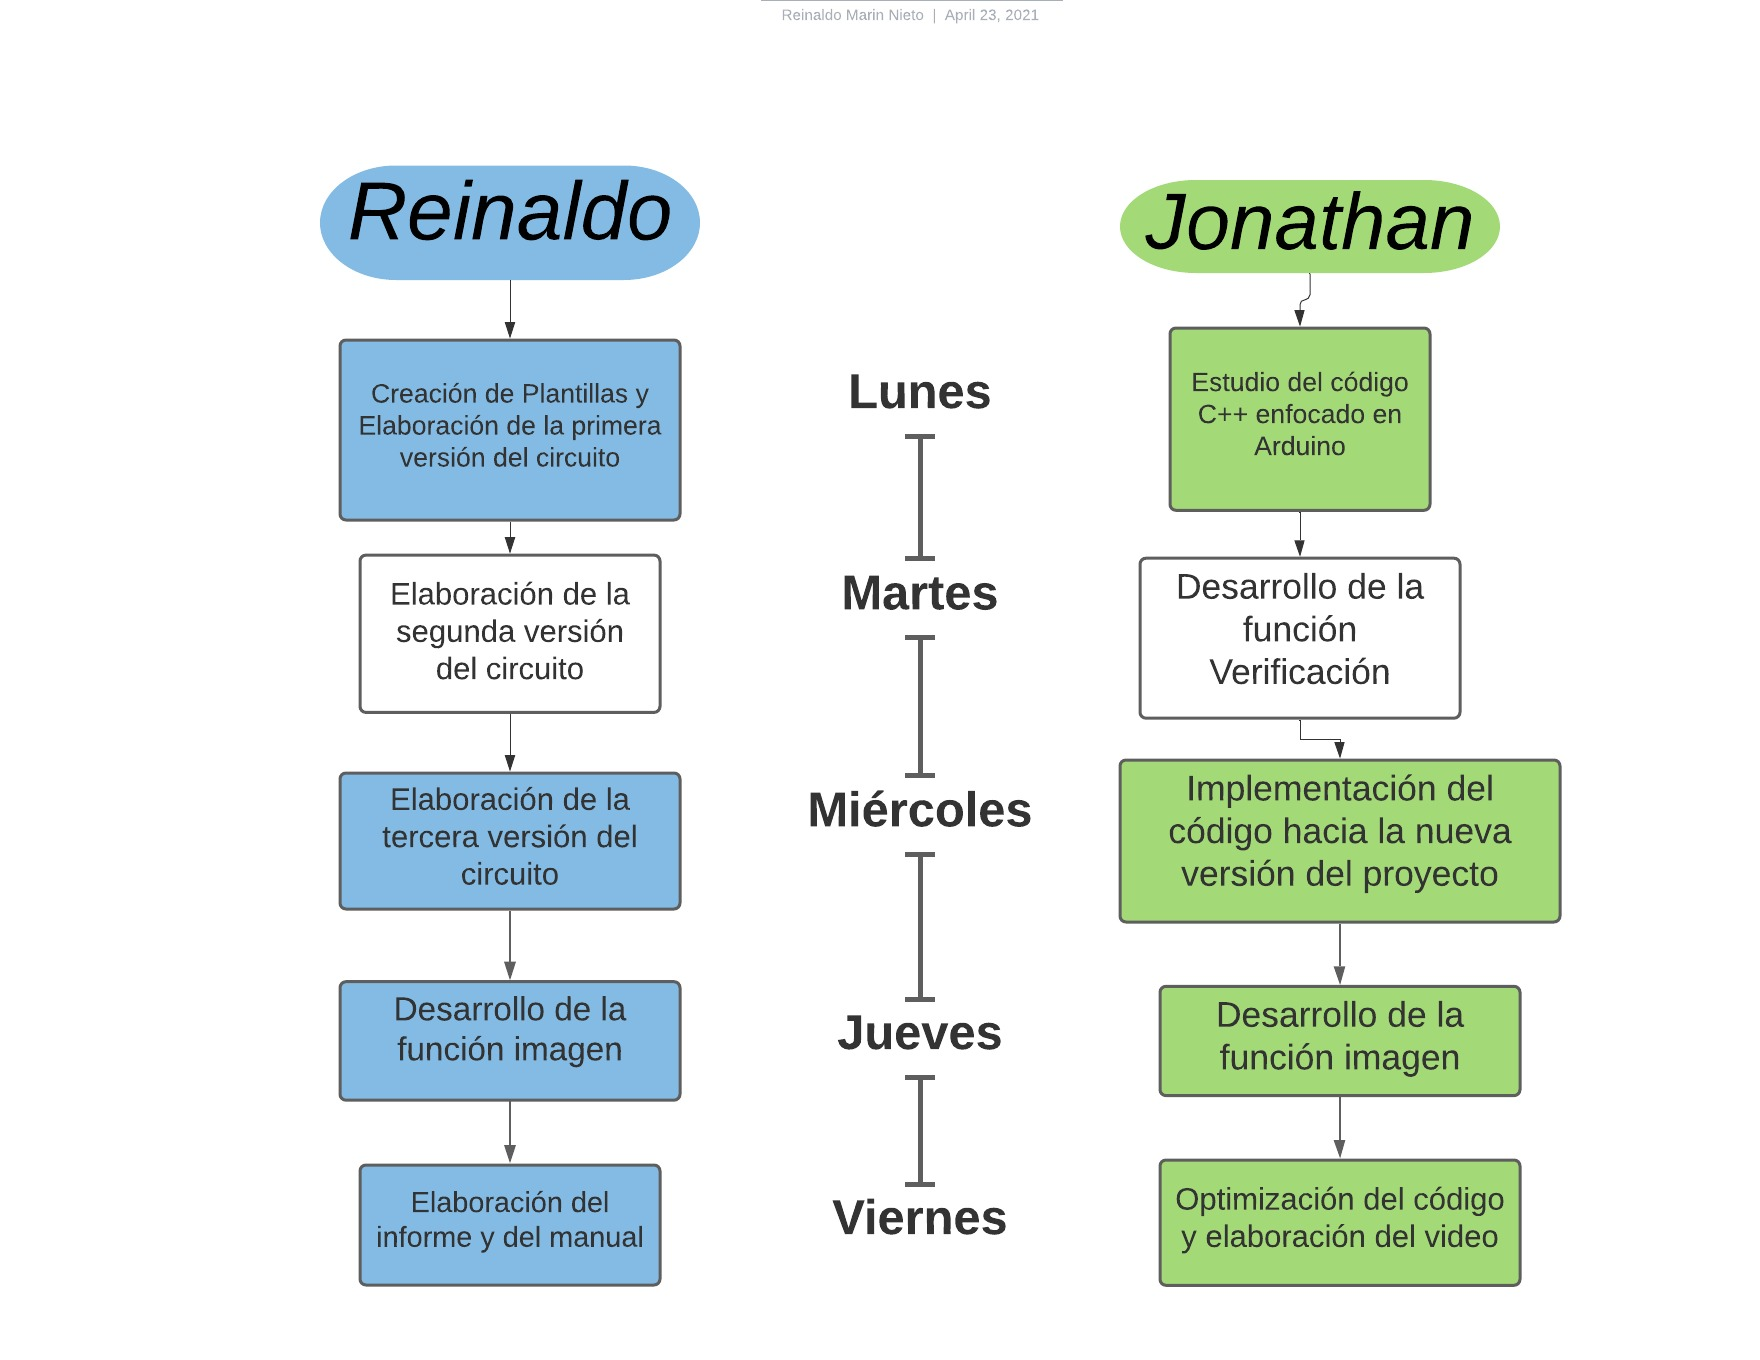
\includegraphics[width=15cm, height=15cm]{Tareas.jpeg}

\section{Problemas presentados en el desarrollo del proyecto} \label{contenido}
Al hacer las primeras dos versiones del proyecto, en donde consideramos sería el más eficiente y fácil de controlar, tuvimos problemas con las especificaciones del ejercicio, en donde se nos ordenaba realizar todo el proyecto con matrices de LEDs 8x8. A causa de ésto, tuvimos que hacer una reconexión completa. Adicionalmente, la plataforma TinkerCad tuvo varias caídas, donde todo nuestro código y una proporción significativa del circuito se eliminaba. Ésto nos hizo perder mucho tiempo, y ocasionó que no lograramos hacer la función publik.
\section{Algoritmo usado} \label{contenido}
\begin{lstlisting}
#define DATA_PIN 11
#define CLOCK_PIN 13
#define SS_PIN_1 10
#define SS_PIN_2 9
int ch[8][8] =
{        
    {1, 1, 1, 1, 1, 1, 1, 1},
    {1, 1, 1, 1, 1, 1, 1, 1},
    {1, 1, 1, 1, 1, 1, 1, 1},
    {1, 1, 1, 1, 1, 1, 1, 1},
    {1, 1, 1, 1, 1, 1, 1, 1},
    {1, 1, 1, 1, 1, 1, 1, 1},
    {1, 1, 1, 1, 1, 1, 1, 1},
    {1, 1, 1, 1, 1, 1, 1, 1}    
};
int matriz_modificable[8][8]{0};
int *puntero_matriz = new int[8]{0};
char col[8]{48,48,48,48,48,48,48,48};
int fila = 1;
char data;
void spi_write_1(unsigned  char cData) {
  shiftOut(DATA_PIN, CLOCK_PIN, MSBFIRST, cData);
  digitalWrite (SS_PIN_1, HIGH);
  digitalWrite (SS_PIN_1, LOW);}
void spi_write_2( unsigned char cData) {
  shiftOut(DATA_PIN, CLOCK_PIN, MSBFIRST, cData);
  digitalWrite (SS_PIN_2, HIGH);
  digitalWrite (SS_PIN_2, LOW);}
void writePosition(int x, int y) {
  spi_write_1(  B00000001 << x );  // COL  
    spi_write_2(~(B00000001 << y )); // ROW
}
  void setup (){  
    pinMode(SS_PIN_1, OUTPUT);
    pinMode(SS_PIN_2, OUTPUT);
    pinMode(DATA_PIN, OUTPUT);
    pinMode(CLOCK_PIN, OUTPUT);
    Serial.begin(9600);
    Serial.println("1. Verificacion de leds");
    Serial.println("2. Crear tu propia imagen");
    spi_write_1(  B00000000);  // COL 
    spi_write_2(~(B00000000)); // ROW   
    }
  void loop(){
    if(Serial.available()==1){
      char t = Serial.read();
      Serial.println(t);
      if(t=='1'){
    	for (int row=0; row <8;row++) 
    	{
  			for (int colu=0; colu <8;colu++) 
  				{if (ch[colu][row] == 1) {
   					writePosition(colu,row);
  					}
                }
        }
      }
    Serial.print("Ingresa opcion");
      if (t =='2'){
        
        while (fila < 8){
          Serial.print("Ingrese la fila que quiere manipular");
          fila = Serial.read();
          Serial.print("Ingrese con 0 y 1 en orden para decidir cualquiere que encienda y cualquiere que se mantenga apagada, 1 para encender, 0 para mantener apagado");
          col = Serial.read();
          for (int i = 0; i<8;i++){
            *(puntero_matriz+i) = col[i] - '0';
          }
          for (int i = 0; i<8; i++){
            matriz_modificable[fila][i] = *(puntero_matriz+i);
          }          
          for (int row = 0; row <8;row++){
                        for (int colu=0; colu<8;colu++){
              if (matriz_modificable[row][colu]== 1){
                writePosition(colu,row);
              }
            }
          }
          Serial.print("Quieres modificar otra fila? Escribe 'Y' en caso que si o 'N' si no");
          data = Serial.read();
          if (data == 'Y');
          else if (data == 'N'){
      		fila = 8;
          }
          while(data != 'Y' && data != 'N'){
            Serial.print("Ingresa un caracter valido, Y para ingresar otra fila, N si quiere salir");
            data = Serial.read();
            if (data == 'Y');
            else if (data == 'N'){
              fila = 8;
            }
          }
        }
      }
    }
  }
\end{lstlisting}
\section{Evolución del algoritmo} \label{contenido}
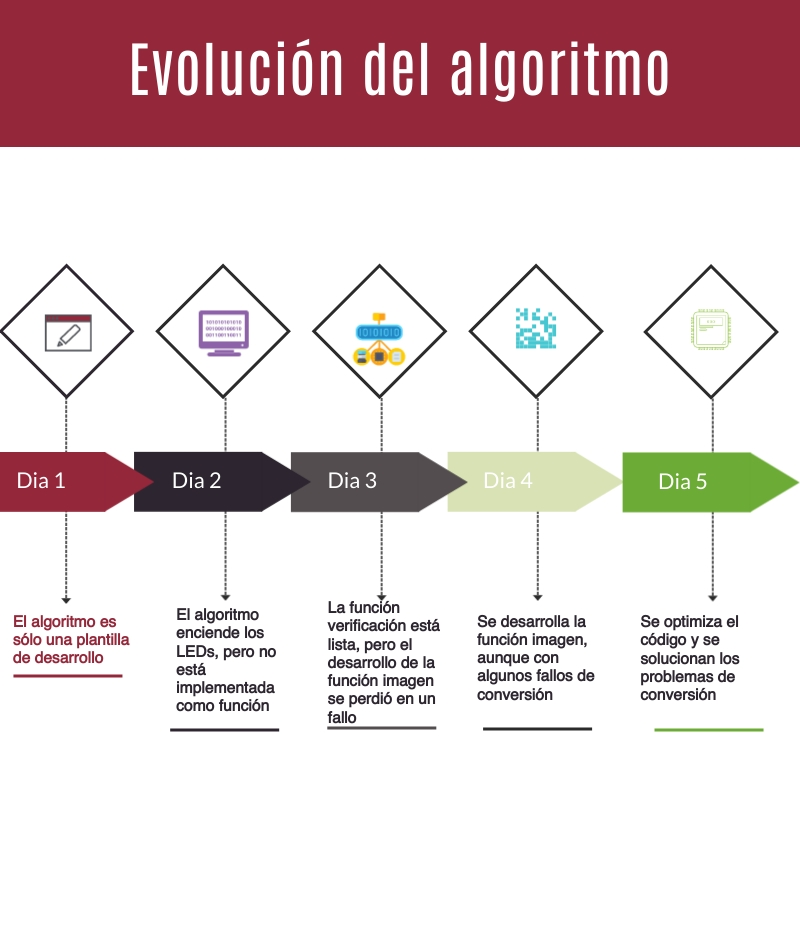
\includegraphics[width=15cm, height=15cm]{Evolucion.jpg}



\end{document}
